\section{Experimentación}

OBLIGATORIO ES LO SIGUIENTE, POR ENUNCIADO

2. Como afecta la calibracion del sistema en el resto de las etapas \\
3. ¿Como impacta la eleccion de las 3 direcciones de iluminacion para el calculo de las normales? \\

\todo[inline]{Experimentacion general pensar mas:  }
\todo[inline]{Diferencias de tiempos EG vs LU, con si y mascara mascara}
\todo[inline]{Mostrar como con diferentes luces obtenemos diferentes normales}
\todo[inline]{Mostrar resultados finales con mismas luces pero propias vs catedra}


1. Comparar las direcciones de iluminacion obtenidas por el metodo de calibracion con las provistas por la catedra \\

Veamos qué tan buena fue nuestra calibración. Dado que la cátedra nos brindó los vectores de luces lo que nos gustaría hacer es comparar ambos. En general, niguna luz quedó \textit{exactamente} igual, pero sí quedaron similares. \\

Dado que es complicado visulizar diferencias entre vectores tridimensionales, analizaremos por un lado el eje $z$ y por el otro los ejes $x$ e $y$. En el siguiente gráfico tomamos para cada luz, los ejes $z$ y calculamos su diferencia. \\

{\centering
    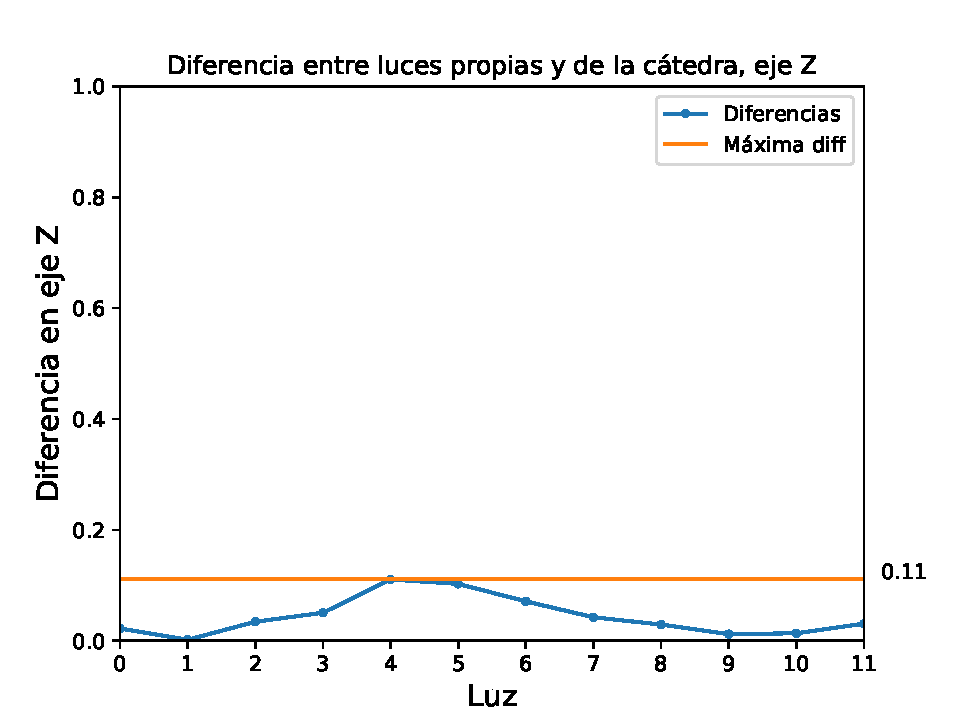
\includegraphics[scale=0.7]{informe/imagenes/lucesEjezDiferencias.pdf} \\
}

Podemos observar que la la diferencia máxima es aproximadamente $0.1$ mientras que la diferencia mínima está cercana a cero (es exactamente $0.001821$ en la luz $1$). Creemos que si bien no es perfecto, es una diferencia aceptable. Dado que todos los vectores son unitarios (pues fueron normalizados) es lógico esperar diferencias entre los ejes x e y. A continuación puede verse el gráfico resultante. Las luces que se corresponden con las propias y las de la cátedra están señaladas con el mismo color. \\

Podemos observar que si bien las diferencias son notorias, todas se encuentran en el mismo rango en inclinación. No hay ninguna que haga cosas extrañas como apuntar en sentido inverso. Creemos que las diferencias no afectarán demasiado el resultado final.

{\centering
    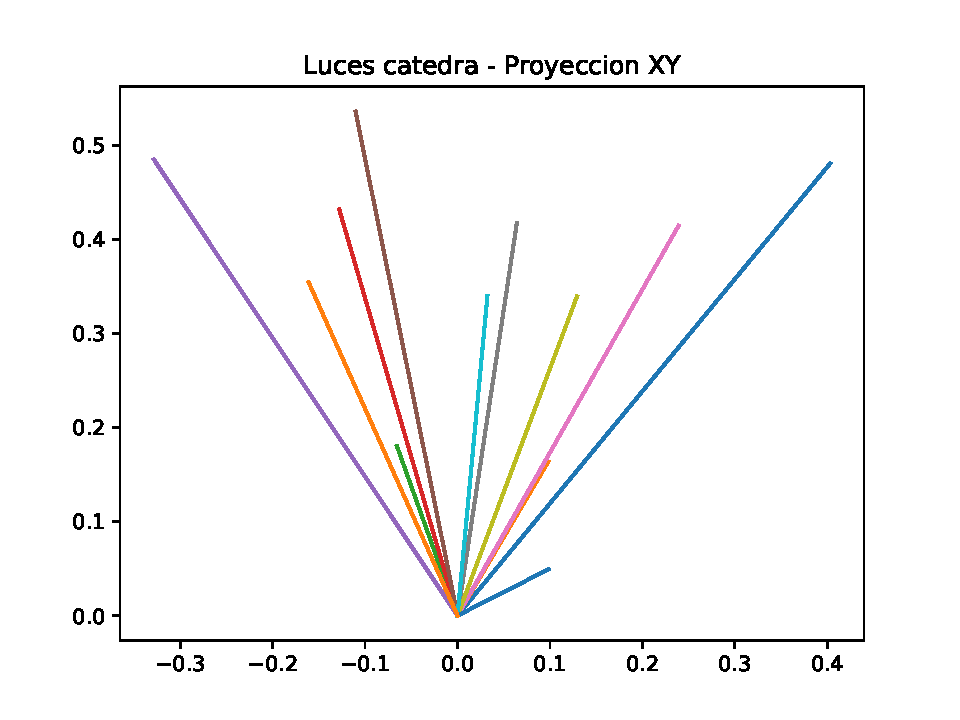
\includegraphics[scale=0.8]{informe/imagenes/lucesCatedraProyeccionXY.pdf} \\
    % \captionof{figure}{Luces de la cátedra en la proyección x,y}
}
{\centering
    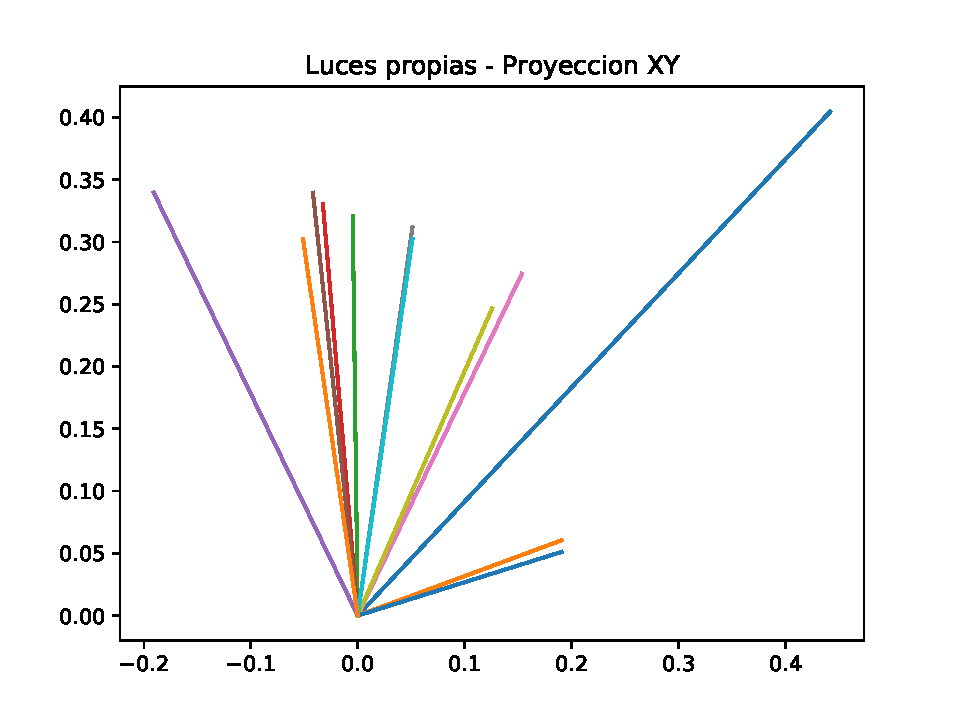
\includegraphics[scale=0.8]{informe/imagenes/lucesPropiasProyeccionXY.pdf} \\
    % \captionof{figure}{Luces propias en la proyección x,y}
}

$ $\newline
